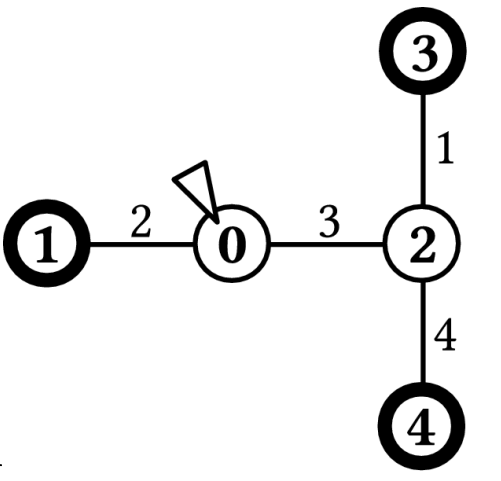
\includegraphics{crocodile1.png}

Consider the first example. Chambers are shown as circles, and corridors connecting them are
shown as lines. Exit chambers are shown as thick-bordered circles.
Benjamas starts at chamber $0$ (marked by a triangle). An optimal
escape plan is the following one:
\begin{itemize}
\item If you ever reach chamber $0$, take the corridor leading to chamber $1$. However, if that corridor is blocked, then take the corridor leading to chamber $2$.
\item If you ever reach chamber $2$, take the corridor leading to chamber $3$. However, if that corridor is blocked, then take the corridor leading to chamber $4$.
\end{itemize}
In the worst case, Benjamas will reach an exit chamber in $7$ units of time. Hence, \t{travel\_plan}
should return $7$.

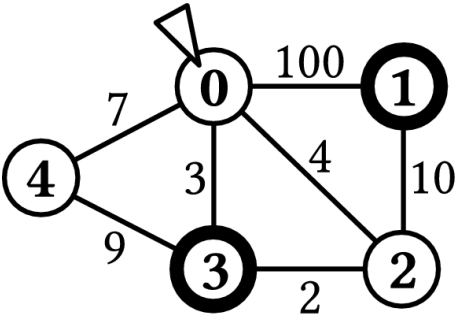
\includegraphics{crocodile2.png}

Here is an optimal escape plan:
\begin{itemize}
\item If you ever reach chamber $0$, take the corridor leading to chamber $3$. However, if that corridor is blocked, then take the corridor leading to chamber $2$.
\item If you ever reach chamber $2$, take the corridor leading to chamber $3$. However, if that corridor is blocked, then take the corridor leading to chamber $1$.
\item Don't bother about chamber $4$; according to this escape plan you cannot possibly reach it.
\end{itemize}
Benjamas will reach one of the exit chambers no later than after $14$ units of time. Therefore,
\t{travel\_plan} should return $14$.
